\documentclass{article}
\usepackage{bbm}
\usepackage{grffile}
\usepackage[utf8]{inputenc}
\usepackage{amsmath,amsfonts,amssymb,amsthm,latexsym,epsfig,epstopdf,titling,url,array}
\usepackage{listings}
\usepackage[normalem]{ulem}
\usepackage{float}
\usepackage{graphicx}
\usepackage{enumerate}

\title{\Huge Creating a Lattice Boltzmann Fluid Solver in TensorFlow}
\author{Vikram Singh}
\date{July 2019}

\setlength{\parindent}{0pt}
\addtolength{\oddsidemargin}{-0.75in}
\addtolength{\evensidemargin}{-0.75in}
\addtolength{\textwidth}{1.5in}

\addtolength{\topmargin}{-0.75in}
\addtolength{\textheight}{1in}

\begin{document}

\maketitle

\section{The Lattice Boltzmann Method}

The Navier-Stokes equations for viscous flow are very complicated and impossible to solve analytically in almost all non-trivial situations. Thus in order to analyse fluid flow in irregular systems, we have to use numerical solvers. One such method is the Lattice Boltzmann Method (LBM) \cite{LBPaper}. This involves simulating the fluid as populations of particles moving on a discrete lattice with velocities along a set of discrete vectors, and simulating collisions at each lattice point \cite{LBBook}.

\section{Potential advantages of TensorFlow for LBM}


Tensorflow is a powerful set of tools that is used extensively in machine learning applications. 
At its core, TensorFlow implements large array operations in a way that  is efficiently parallelisable across all available CPU cores or a GPU.
Since it automatically parallelises large array operations, it can potentially provide speed improvements over even highly optimised numerical libraries such as Numpy.

Many of the operations of a Lattice Boltzmann solver are performed on large arrays that represent a space of lattice points, and so the efficiency of Tensorflow could potentially be used to improve the speed of a solver.
In particular, the calculation of macroscopic variables, and the collision with an obstacle, can be expressed as convolutions of an array, which is implemented very well in TensorFlow.

In this project I investigated the potential improvements of TensorFlow over Numpy.

\section{Analysis}

To analyse the benefits of TensorFlow, I implemented two versions of the Lattice Boltzmann Solver - one using only Numpy, and one using Tensorflow to perform all of the lattice calculations. My code for these solvers is available at (\url{https://github.com/vikram8128/PythonLatticeBoltzmann}).

I then performed a number of tests to analyse the performance of both of these solvers.

\subsection{Methodology}

My tests consisted of 6 different simulations, using both the TensorFlow and Numpy solvers. These were:

\begin{enumerate}
    \item Flow around a cylinder with low viscosity ($420\times180$ lattice points)
    \item Flow around a cylinder with high viscosity ($420\times180$ lattice points)
    \item Flow around an airfoil ($420\times180$ lattice points)
    \item Flow through a narrowing pipe ($420\times180$ lattice points)
    \item Flow through a bending pipe ($1000\times452$ lattice points)
    \item flow in a lid driven cavity ($180\times180$ lattice points)
\end{enumerate}

The simulations ran for 20000 timesteps, producing .png output every 100 timesteps. Figure 1 contains a sequence of images from an extended version of simulation 2 (flow around a cylinder with high viscosity). The complete animations of each of the simulations are available in the github repository. Each of these simulations was run on an Intel Skylake server, with 32 CPU cores.

\begin{figure}[H] 
	\centering
	\label{videoCuts}
	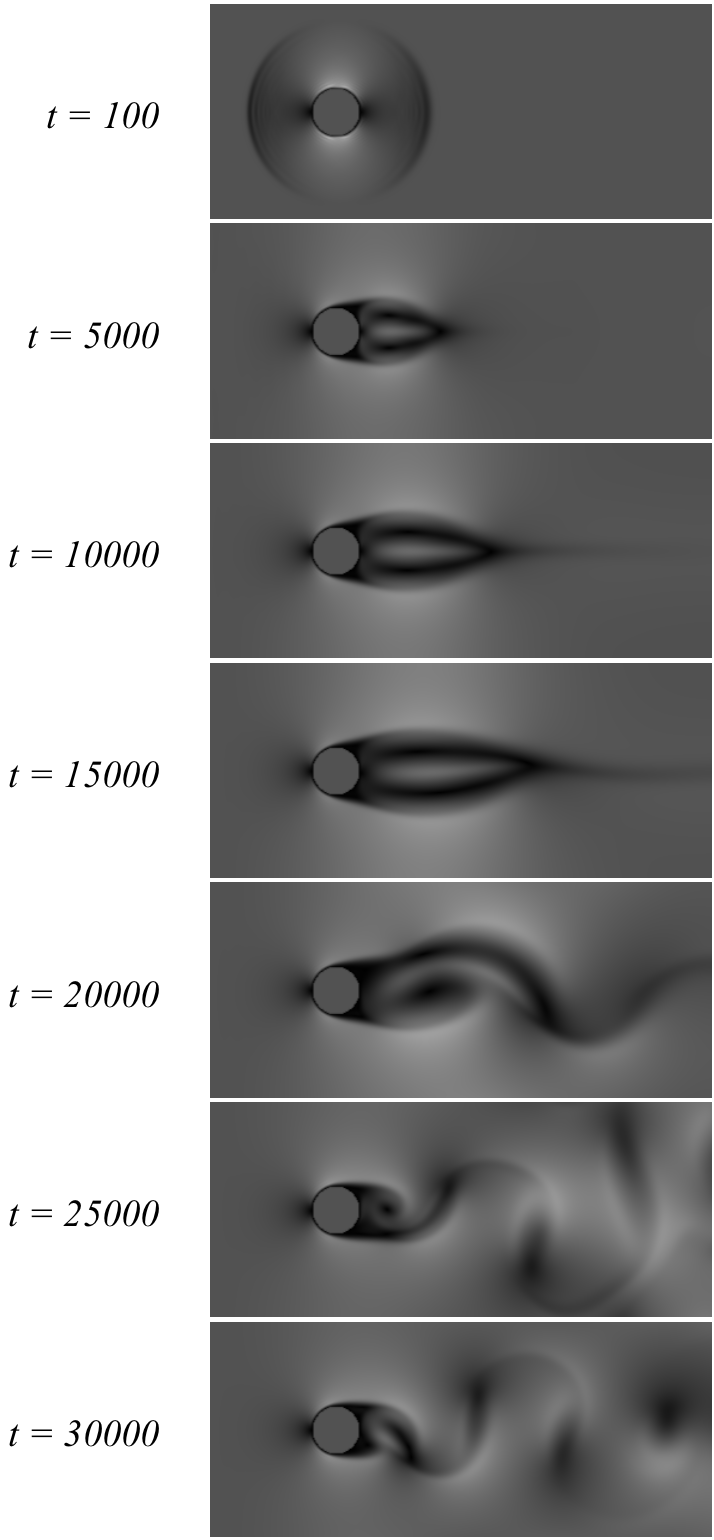
\includegraphics[width=3in]{Diagrams/CylinderFlowImages.png}
	\caption{Intermediate image outputs from simulation 2}
\end{figure}

\subsection{Results}

The simulations were run 3 times each, and the mean real times are shown in Table 1. 

\begin{table}[H]
\caption{The wallclock times in seconds taken by each simulation}
\begin{center}
\begin{tabular}{c||c|c|c|c|c|c}
\emph{Simulation} & 1 & 2 & 3 & 4 & 5 & 6\\
\hline
\hline
\emph{Numpy} & 316 & 311 & 319 & 1565 & 4043 & 615 \\
\hline
\emph{TensorFlow} & 198 & 198 & 198 & 199 & 708 & 122 \\
\hline
\end{tabular}
\end{center}
\end{table}

In these results, I assumed a conservative 10\% uncertainty in the time (observed error was around 2\%). From this, I created the plot in figure 2.

\begin{figure}[H] 
	\centering
	\label{timegraph}
	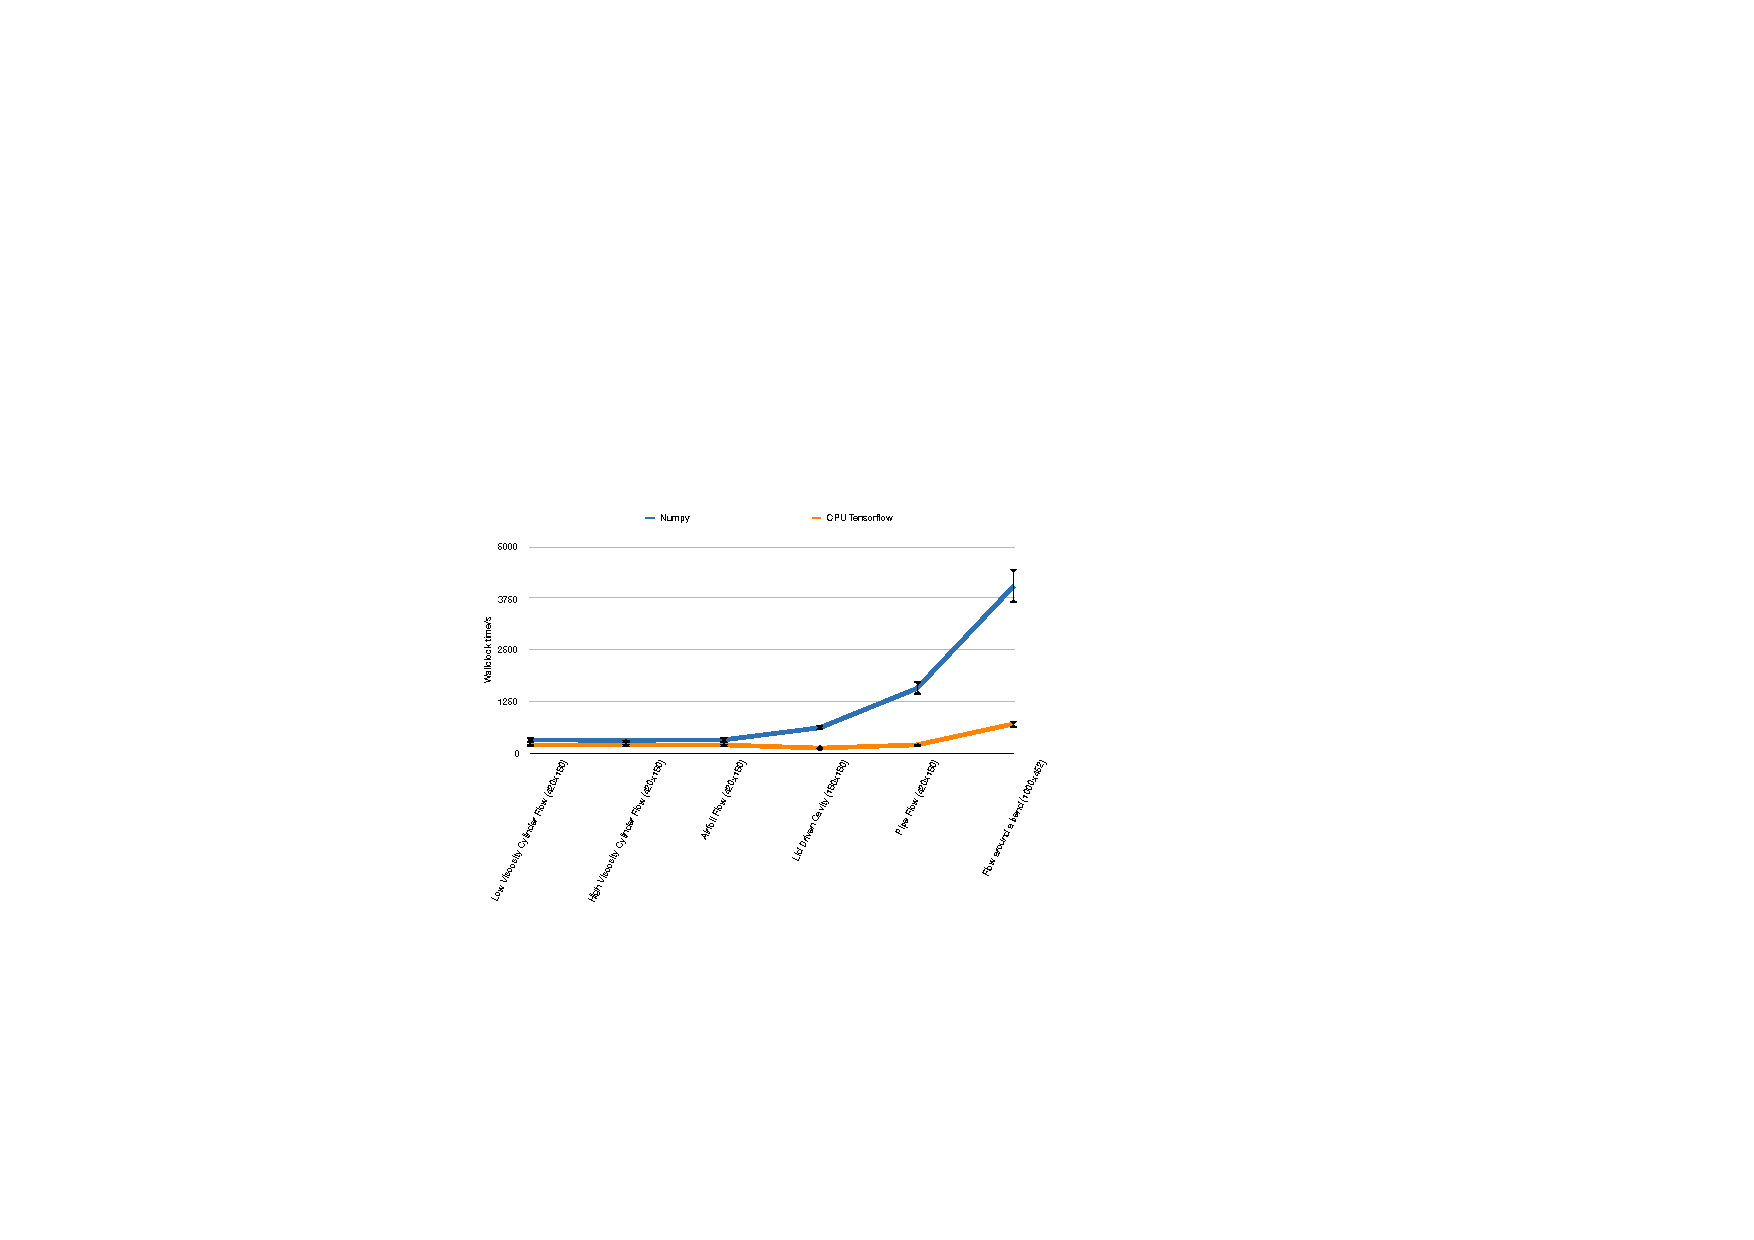
\includegraphics[width=5in]{Diagrams/TimeGraph.pdf}
	\caption{Runtimes of simulations}
\end{figure}

In addition, I calculated the rate of cell updates (in Megahertz) for each of the simulations, which is shown in table 2.

\begin{table}[H]
\caption{Cell updates per second (MHz) for each of the simulations}
\begin{center}
\begin{tabular}{c||c|c|c|c|c|c}
\emph{Simulation} & 1 & 2 & 3 & 4 & 5 & 6\\
\hline
\hline
\emph{Numpy} & 4.78 & 4.86 & 4.74 & 0.966 & 2.24 & 1.05 \\
\hline
\emph{TensorFlow} & 7.64 & 7.64 & 7.64 & 7.60 & 12.8 & 5.31 \\
\hline
\end{tabular}
\end{center}
\end{table}

Again assuming 10\% uncertainty in this data, we get the plot of cell update frequency in figure 3.

\begin{figure}[H] 
	\centering
	\label{freqgraph}
	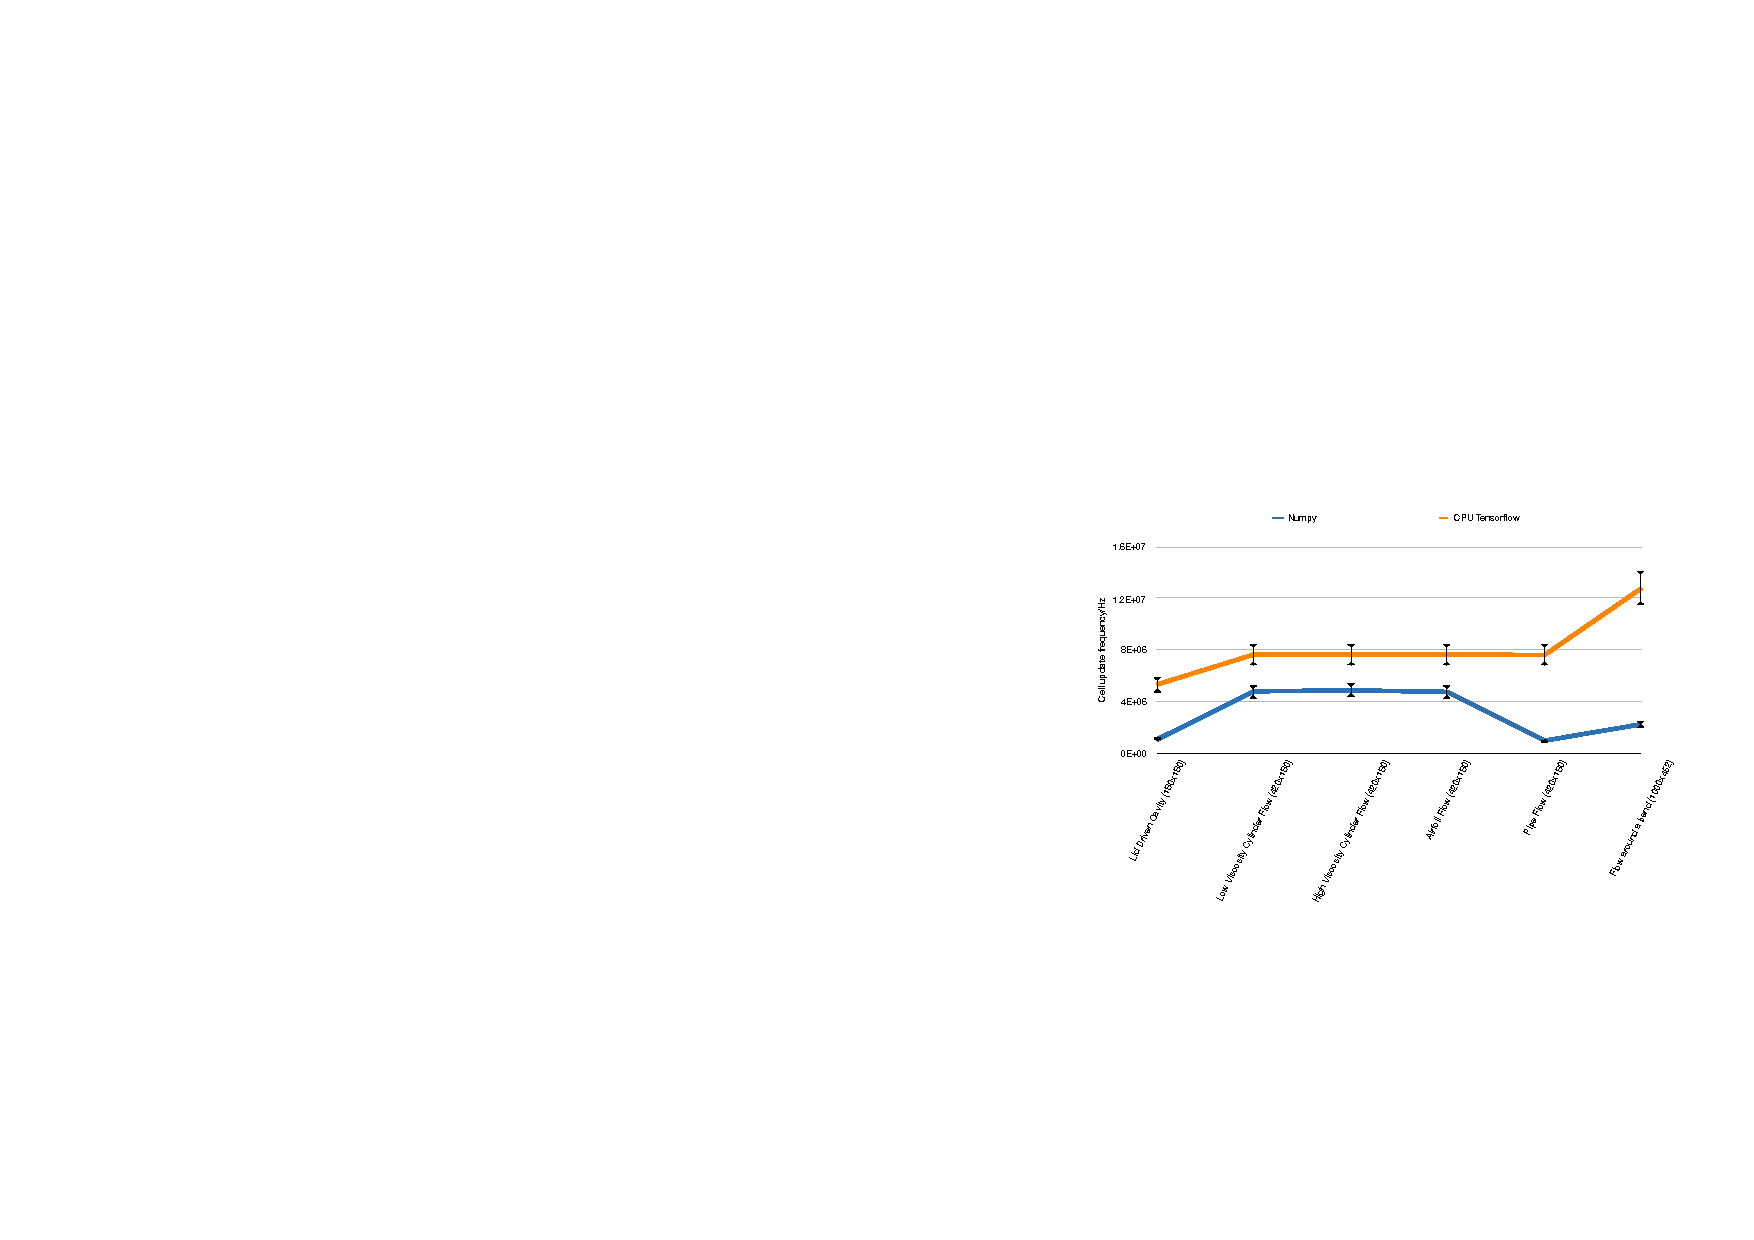
\includegraphics[width=5in]{Diagrams/FreqGraph.pdf}
	\caption{Cell update frequencies of the simulations}
\end{figure}

\subsection{Conclusions}

We observe that TensorFlow consistently outperforms Numpy, but the improvement factor is not constant. In the simulations of flow in a narrowing pipe, flow in a lid driven cavity and flow in a bending pipe, TensorFlow is faster by a factor of about 5 times, as opposed to about 1.5 in the other three simulations. The simulations where there is a larger improvement have larger areas of obstacle, and in addition, the bending pipe simulation has a much larger lattice. We can conclude that TensorFlow scales much better than Numpy with an increased lattice size, and an increased area of obstacle. The improved parallelisation that is implemented in TensorFlow gives a large improvement in speed of the Solver, which scales well with size. This improvement could be very useful for even larger fluid dynamics simulations such as in industrial applications.

\section{Next Steps}

While this project has provided some useful results, there are some areas that I have not explored. Mainly, I did not study how the performance of the models translates to 3D models, where the factor of improvement that TensorFlow provides could be different to the 2D simulations that I examined. Additionally, I only used CPUs to run my TensorFlow simulations. Adapting them slightly to run on GPUs may give a further speed improvement. However, GPU TensorFlow does not support the (\emph{roll}) operation that is used extensively, so this would have to be implemented manually. Both expanding the solvers to 3D, and running the TensorFlow solvers on GPUs would be potentially quite informative, and these require further investigation.



\addcontentsline{toc}{section}{References}
\begin{thebibliography}{99}

\bibitem{LBPaper} Chen, Shiyi, Doolen, Gary D. (1998). \emph{LATTICE BOLTZMANN METHOD FOR FLUID FLOWS} Annual Review of Fluid Mechanics 30 (1): 329–364 doi:10.1146/annurev.fluid.30.1.329

\bibitem{LBBook} Alexander J. Wagner (2008) \emph{A Practical Introduction to the Lattice Boltzmann Method}, North Dakota State University

\bibitem{TFDocs} TensorFlow Documentation (\url{www.tensorflow.org/api_docs/python/})

\end{thebibliography}

\end{document}